\section{Grafisk bruger interface}\label{GUI_design}
\textit{Dette afsnit omhandler design, implementering og test af GUI til visualisering af de udførte aktiviteter.}

\subsection{Design}
GUI benyttes i dette projekt til at motivere børn til en mere aktiv hverdag. Dette gøres ud fra \secref{motivation_boern}, hvor det beskrives, at børn motiveres gennem succesoplevelser. GUI designes med henblik på at give børnene et overblik over, hvor lang tid de har udført en given aktivitet, og hvor mange point de har optjent som følge af dette. Pointene vægtes ud fra aktivitetstypen og varigheden heraf.

Data fra gyroskopet sendes til MATLAB som tre bytes. Først sendes en identifikation (ID) på én byte, og derefter gyroskopdata i en pakke bestående af low byte og high byte. Arrayet af data, som modtages fra gyroskopet, er dermed: [ID~-~Gyroskopdata(low byte)~-~Gyroskopdata(highbyte)]. Data fra accelerometeret sendes som i alt fem bytes. Først sendes et ID på én byte, hvorefter tiden mellem to peaks sendes som en pakke bestående af low byte og high byte. Peakværdien sendes i en pakke, som ligeledes bestående af low byte og high byte. Arrayet af data fra accelerometeret er dermed: [ID~-~Tid(low byte)~-~Tid(high byte)~-~Peak(low byte)~-~Peak(high byte)]. Den første byte i begge arrays er altså et ID, som angiver hvorvidt dataet kommer fra accelerometeret eller gyroskopet, som det ses på \figref{fig:GUI}. ID'et for accelerometeret er 2, mens ID'et for gyroskopet er 3.\\
Hvis MATLAB registrerer accelerometerets ID, findes peakværdien til detektion af gang og løb, som en pakke bestående af fjerde og femte byte i arrayet. Den modtagende peakværdi videregiver informationer om, hvorvidt tidsvariablen skal adderes til gang eller løb. På anden og tredje plads findes en pakke af tidsenheden, som er resultat af varighed siden sidste detekterede peak. Er amplitudeværdien for peaket mellem 50 og 400 skal varigheden adderes i tidsvariablen for gang, og er den lig med eller over 400, skal den overføres til tidsvariablen for løb.\\
Registreres gyroskopets ID som den første byte, påbegyndes databehandlingen for pakken bestående af anden og tredje byte. Denne databehandling foregår i MATLAB, som beskrevet i \secref{sec:algocykel}. Er resultatet over 70\%, overføres fire sekunder til tidsvariablen for cykling til GUIen.

Hver aktivitet belønnes forskelligt, hvilket skyldes at cykling og løb har et højere intensitetsniveau end gang. Herved stiger pulsen gennem disse aktiviteter, der giver et andet fysiologisk udbytte end aktivitet udført ved lav intensitet. Derfor omregnes tiden til point ved at multiplicere tiden for løb med 3, for cykling med 2 og for gang med 1, da det vurderes at løb har størst intensitet og gang har lavest.\\ 
Pointene visualiseres i GUI ud for den enkelte aktivitet, hvorved barnet kan se, hvor mange point der er optjent. For at give barnet bedre visualisering af udført aktivitet over en periode summeres pointene for hver dag og plottes i en graf. Pointene vises grafisk som tre søjler for hver aktivitet i individuelle farver. Barnet kan dermed se, hvor stor en del hver aktivitet har udgjort af dagens totale antal point.  
\begin{figure}[H]
	\centering
	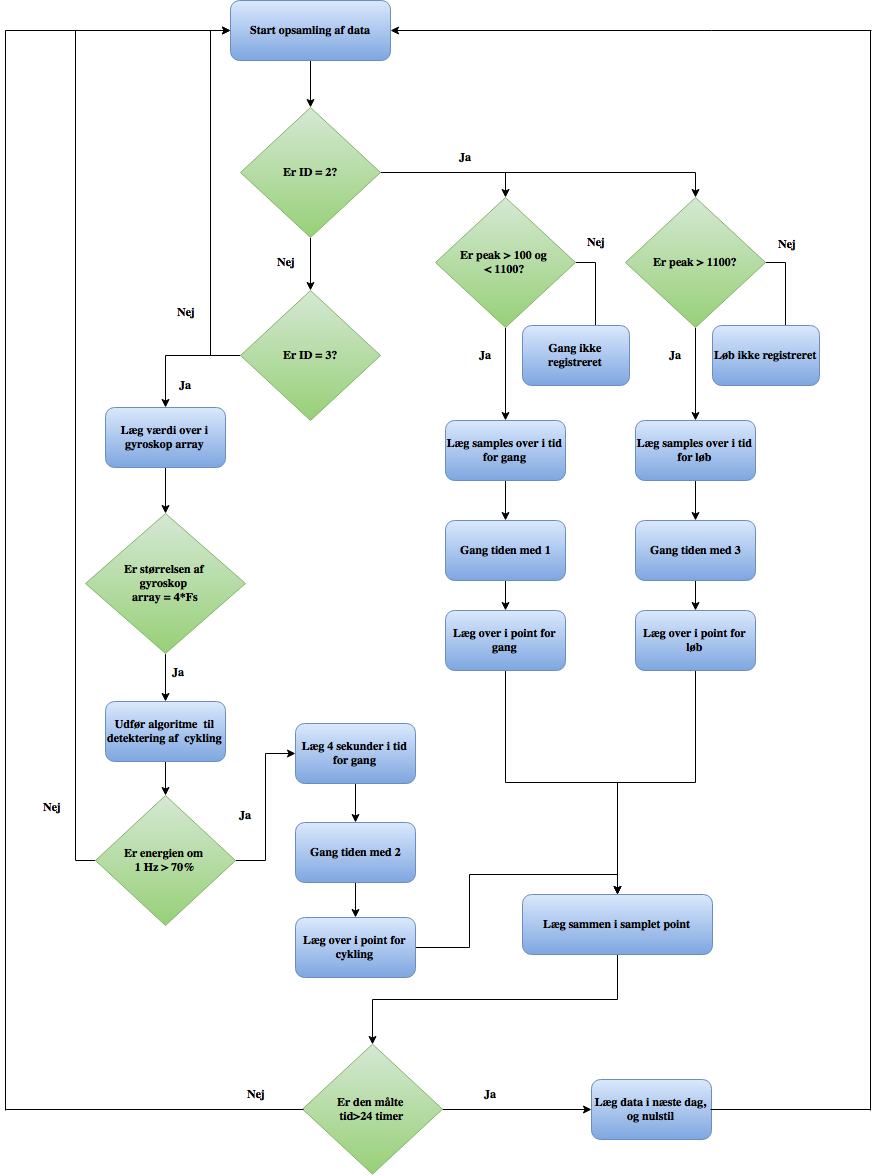
\includegraphics[scale=0.4]{figures/cDesign/pseudo_GUI.png}
	\caption{På figuren ses et flowchart, der gennemgår hvorledes resultaterne fra de forskellige algoritmer behandles af GUI.}
	\label{fig:GUI}
\end{figure}\vspace{-.25cm}

\subsection{Implementering}
GUI implementeres ved at skabe en figur i MATLAB, hvori henholdsvis brugerens tid og point printes i en tabel for hver aktivitet. Derudover fremkommer en tabel, som visualiserer dagens samlede aktiviteter. Hertil plottes et søjlediagram over brugerens point for dagen, som plottes i tre forskellige søjler og farver alt efter aktiviteten.

Programmet starter idet der trykkes 'Run' i MATLAB, hvorved indhentning af data fra mikrokontrolleren begynder. Programmet benytter ID'et for data til at adskille accelerometerdata og gyroskopdata. Er den første byte 2 i det indhentede array, registreres mikrokontrollerens data som værende accelerometerdata. Den anden og tredje byte i arrayet er en repræsentation af en pakke for hvor mange samples der er mellem hvert peak. Denne skal omregnes til sekunder og overføres til tidsvariablen for den pågældende aktivitet. Omregning udføres som det ses i \eqref{eq:tidsvariabel}. Den anden og tredje byte angiver peakværdien, hvilken indikerer om aktiviteten er gang eller løb. \\
Er den første byte i arrayet 3, registrerer GUI data som værende data fra gyroskopet. Den anden og tredje byte repræsenterer en pakke i arrayet, som overføres til et nyt array, der behandles som beskrevet i \secref{sec:algocykel}. En tidsvariabel på fire sekunder overføres derefter til cykling, hvis databehandlingen viser at energien omkring den maksimale peak summeret fra $\pm$1~Hz er over 70\%. 
\begin{equation}
Tidsvariabel = \frac{Samples}{Samplingsfrekvens}
\label{eq:tidsvariabel}
\end{equation}
'Tidsvariablen' fra \eqref{eq:tidsvariabel} benyttes til at udregne point for aktiviteterne. Dette gøres ved at multiplicere med de tidligere nævnte værdier opnået som følge af aktivitetstypen. Dette ses i \eqref{eq:pointvariabel}. 
\begin{equation}
Pointvariabel = Tidsvariabel \cdot Aktivitetspoint
\label{eq:pointvariabel}
\end{equation}
'Tidsvariablen' og 'pointvariable' for de enkelte aktiviteter overføres til forskellige 'static text felter'. Disse tilhører henholdsvis point og tid for de tre forskellige aktivitetstyper. Ydermere er der to forskellige 'static text felter', hvor der i den ene samles 'tidsvariablerne' for hele dagen, og i den anden samles point opnået gennem hele dagen. \\
Der implementeres et søjlediagram, hvor data plottes. I denne samles point fra gang, løb og cykling, som plottes ved siden af hinanden med forskellige farver. Dette gør det muligt at se, hvilke aktiviteter der er udført, og hvor mange point der samlet er optjent for en dag. I programmet er der aktiveret en timer, som gør det muligt at skifte til en ny dag efter 24~timer. Ved begyndelse på en ny dag nulstilles alle variabler, og der plottes i den næste dag.\\ 
Afslutningsvist kan programmet stoppes ved at der trykkes 'Q' på tastaturet. Herved stoppes dataindhentningen og optællingen af aktivitetstid samt tilhørende point, hvorfor figuren fryses og derefter lukkes. 

\subsection{Test}
Testen udføres på baggrund af de opstillede krav og tilhørende afvigelser opstillet i \secref{krav_GUI}, som beskriver, at GUIen skal:
\begin{itemize}
	\item Kunne visualisere tidsforbruget, intensitet og point opnået ved henholdsvis gang, løb og cykling. Der accepteres inden andre former for visualisering.
\end{itemize}

Testen udføres ved at indsende kendte værdier, hvoraf hver aktivitet kan testes individuelt i forhold til multiplikation som følge af aktivitetstype. I testen indsendes et datasæt med simuleret input fra algoritmen, som skal ramme tærskelværdien og derved optælles som de forskellige aktiviteter. For gang indsendes [2~-~473(low byte)~-~473(high byte)~-~1050(low byte)~-~1050(high byte)], for løb indsendes [2~-~473(low byte)~-~473(high byte)~-~1150(low byte)~-~1150(high byte)] og for cykling indsendes [3~-~Simuleret\_sinus(low byte)~-~simuleret\_sinus(high byte)]. Gang og løb simuleres samtidig med et sekunds delay gennem forskellige arrays fra PSoC. Den simulerede sinus laves i MATLAB, hvorfra det direkte benyttes i GUI. Alt det simulerede data indsendes i MATLAB, hvor det hver har en varighed af 30~sekunder.

Resultatet af GUIs design medfører, at forskellige aktivitetsformer bidrager til et forskelligt antal point. Resultatet af testen ses i \tabref{test:GUI} og på \figref{fig:GUI2}. Derudover visualiseres point for de forskellige aktiviteter i et søjlediagram, hvilket ligeledes kan ses på \figref{fig:GUI2}.
\begin{table}[H]
	\centering
	\begin{tabular}{ccccc}
		\hline
		\rowcolor[HTML]{C0C0C0} 
		Aktivitet & \begin{tabular}[c]{@{}c@{}} Forventet tid \\ {[}s{]} \end{tabular} & \begin{tabular}[c]{@{}c@{}} Optalt tid \\ {[}s{]} \end{tabular}	& \begin{tabular}[c]{@{}c@{}} Forventet \\ antal point \end{tabular} & \begin{tabular}[c]{@{}c@{}} Optalt \\ antal point \end{tabular} \\ \hline
		Gang 	& 30 & 30 &  30 & 30  \\ \hline
		Løb 	& 30 & 30 & 90 & 90 \\ \hline
		Cykling & 30 & 30 & 60 & 60 \\ \hline
	\end{tabular}
	\caption{I tabellen ses sammenhængen mellem henholdsvis forventet tid og optalt tid samt forventet antal point og optalt antal point som resultat af det indsendte simulerede data.}
	\label{test:GUI}
\end{table}\vspace{-.25cm}

\begin{figure}[H]
	\centering
	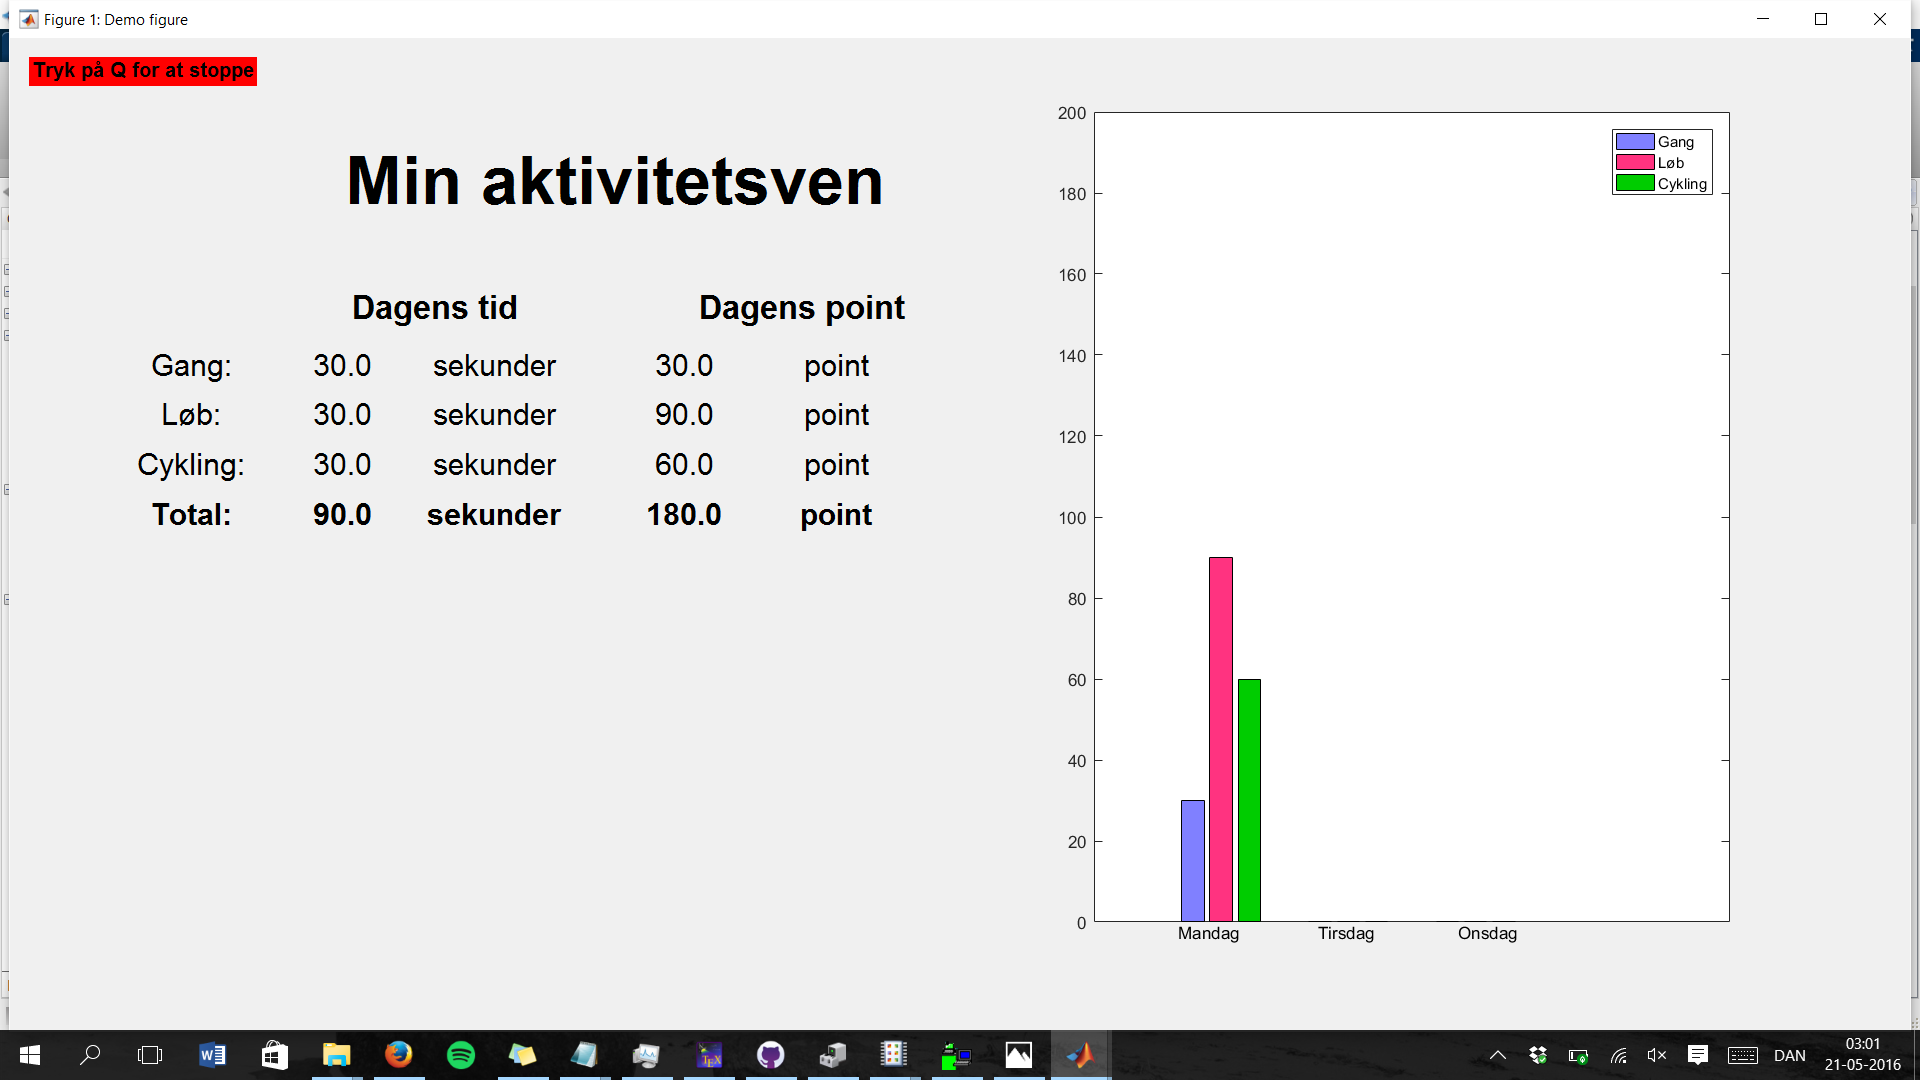
\includegraphics[scale=0.4]{figures/cDesign/test_GUI.png}
	\caption{På figuren ses et udklip af GUI, hvor en simulering af aktiviteterne gang, løb og cykling visualiseres. Aktiviteternes samlede antal point og udført varighed ses på figuren.}
	\label{fig:GUI2}
\end{figure}\vspace{-.25cm}
Som resultat af testen omhandlende GUI kan det konkluderes, at denne opfylder kravene heraf. GUI er i stand til at visualisere tidsforbruget samt antal opnåede point for alle aktiviteterne. GUI opdaterer kontinuert i testen hver gang et nyt input bliver indsendt, hvoraf kravet vedrørende opdatering af GUI mindst hvert femtende minut ligeledes er opfyldt.